%==============================================================================
%  Final-Year Internship Report — Cloud-Native 5G Core Network
%  PART ONE / CHAPTER 1 : General Presentation of the Project
%
%  Author : Malek Aziz Hassayoun     Institution : ESPRIT     Date : June 2026
%
%  Compile:  pdflatex report.tex   (run twice for the ToC / cross-references)
%  Requires: listings, xcolor, hyperref, booktabs, tikz, geometry, fancyhdr,
%            amssymb, tabularx, longtable, enumitem, titlesec
%
%  NOTE: This is Part One. Subsequent chapters (design, implementation,
%  testing, deployment, results) will be added incrementally after development.
%==============================================================================
\documentclass[11pt,a4paper]{report}

%------------------------------------------------------------------ packages
\usepackage[utf8]{inputenc}
\usepackage[T1]{fontenc}
\usepackage[english]{babel}
\usepackage{lmodern}
\usepackage{amssymb}
\usepackage[a4paper,margin=2.5cm]{geometry}
\usepackage{graphicx}
\usepackage{booktabs}
\usepackage{longtable}
\usepackage{array}
\usepackage{tabularx}
\usepackage{xcolor}
\usepackage{listings}
\usepackage{enumitem}
\usepackage{fancyhdr}
\usepackage{titlesec}
\usepackage{tikz}
\usetikzlibrary{shapes.geometric, arrows.meta, positioning, fit, backgrounds}
\usepackage[hidelinks]{hyperref}
\hypersetup{colorlinks=true, linkcolor=blue!55!black, urlcolor=blue!55!black,
            citecolor=blue!55!black}

%------------------------------------------------------------------ colours
\definecolor{codebg}{RGB}{245,245,245}
\definecolor{codekw}{RGB}{0,0,180}
\definecolor{codecmt}{RGB}{0,128,0}
\definecolor{codestr}{RGB}{163,21,21}
\definecolor{accent}{RGB}{20,90,160}
\definecolor{accent2}{RGB}{150,40,90}
\definecolor{light}{RGB}{232,240,250}
\definecolor{light2}{RGB}{250,235,242}

%------------------------------------------------------------------ listings
\lstset{
  backgroundcolor=\color{codebg},
  basicstyle=\ttfamily\footnotesize,
  keywordstyle=\color{codekw}\bfseries,
  commentstyle=\color{codecmt}\itshape,
  stringstyle=\color{codestr},
  numberstyle=\tiny\color{gray},
  breaklines=true,
  showstringspaces=false,
  frame=single,
  rulecolor=\color{gray!40},
  captionpos=b,
  tabsize=2,
  numbers=left,
  numbersep=6pt,
}
\lstdefinelanguage{yaml}{
  keywords={true,false,null},
  comment=[l]{\#},
  morestring=[b]',
  morestring=[b]",
}

%------------------------------------------------------------------ headers
\pagestyle{fancy}
\fancyhf{}
\fancyhead[L]{\small\itshape Cloud-Native 5G Core Network}
\fancyhead[R]{\small\itshape Chapter 1 — General Presentation}
\fancyfoot[L]{\scriptsize ESPRIT — June 2026 \quad|\quad Confidential}
\fancyfoot[R]{\scriptsize Malek Aziz Hassayoun}
\fancyfoot[C]{\small\thepage}
\renewcommand{\headrulewidth}{0.4pt}
\renewcommand{\footrulewidth}{0.2pt}

\titleformat{\chapter}[display]
  {\normalfont\huge\bfseries\color{accent}}
  {\chaptertitlename\ \thechapter}{10pt}{\Huge}

%------------------------------------------------------------------ shortcuts
\newcommand{\code}[1]{\texttt{\small #1}}
\newcommand{\nf}[1]{\textsc{#1}}
\newcommand{\yes}{\textcolor{green!55!black}{\checkmark}}
\newcommand{\no}{\textcolor{red!70!black}{\ding{55}}}
\usepackage{pifont}

%==============================================================================
\begin{document}

%------------------------------------------------------------------ title page
\begin{titlepage}
  \centering
  \vspace*{0.8cm}
  {\large\scshape ESPRIT — École Supérieure Privée d'Ingénierie et de Technologies\par}
  \vspace{0.3cm}
  {\normalsize Final-Year Engineering Internship Report\par}
  \vspace{1.4cm}
  \rule{\linewidth}{0.6pt}\\[0.5cm]
  {\Huge\bfseries\color{accent} Cloud-Native 5G Core Network\par}
  \vspace{0.5cm}
  {\large A Security-Hardened, Roaming-Aware and Observable\\
   Service-Based 5G Core with Automated Conformance Testing\par}
  \rule{\linewidth}{0.6pt}\\[1.4cm]

  {\Large\bfseries Part One --- Chapter 1\\[0.2cm]
   General Presentation of the Project\par}
  \vspace{1.8cm}

  \begin{tabular}{rl}
    \toprule
    \textbf{Candidate}   & Malek Aziz Hassayoun\\
    \textbf{Institution} & ESPRIT\\
    \textbf{Period}      & June 2026 (final-year internship)\\
    \textbf{Domain}      & Telecom R\&D $\cdot$ Network Security $\cdot$ Cloud-Native Systems\\
    \textbf{Standards}   & 3GPP Release 15/16 $\cdot$ TS 23.501 / 23.502 / 33.501\\
    \bottomrule
  \end{tabular}

  \vfill
  {\small\itshape This document is Part One of the report. Design, implementation,
   testing, deployment and results chapters are added incrementally after each
   development phase.\par}
  \vspace{0.4cm}
  {\scriptsize Confidential — ESPRIT — June 2026\par}
\end{titlepage}

%------------------------------------------------------------------ ToC
\tableofcontents
\listoffigures
\listoftables
\clearpage

%==============================================================================
\chapter{General Presentation of the Project}
%==============================================================================

\section*{Chapter Introduction}
\addcontentsline{toc}{section}{Chapter Introduction}
This first chapter presents the general framework of the internship. It defines
the project's ambition, situates it within the 5G Core (5GC) landscape, states the
engineering problems it tackles, and describes the extended system architecture ---
including the \textbf{zero-trust security}, \textbf{roaming}, \textbf{anomaly
detection}, \textbf{observability / business-intelligence}, and \textbf{automated
conformance testing} layers that differentiate this work from a vanilla open-source
core. The chapter closes with the methodology, technical environment, expected
deliverables, targeted competencies, and a feasibility and scope analysis. It is the
foundation on which the subsequent, development-driven chapters are built.

%==============================================================================
\section{Executive Summary}
This project proposes the design, implementation, security hardening, and validation
of a cloud-native \textbf{5G Core (5GC)} network prototype. Going beyond a standard
educational implementation, it introduces four differentiating layers that are not
found --- or not enabled by default --- in mainstream open-source 5G cores.

\begin{table}[h]
\centering
\renewcommand{\arraystretch}{1.35}
\begin{tabularx}{\linewidth}{@{}c l X@{}}
\toprule
\textbf{\#} & \textbf{Layer} & \textbf{What it adds}\\
\midrule
01 & \textbf{Zero-Trust Security} &
  Mutual TLS on all SBI interfaces, certificate-based NF identity, and network-policy
  enforcement between micro-services --- capabilities absent from open5GS and free5GC by
  default.\\
02 & \textbf{Roaming \& Interconnect} &
  \textbf{SEPP}-based inter-PLMN roaming over a secured \textbf{N32} interface (topology
  hiding, message protection), supporting home-routed and local-breakout roaming ---
  rarely implemented end-to-end in OSS cores.\\
03 & \textbf{Anomaly Detection Engine} &
  Lightweight ML/statistical model trained on 5G signalling patterns to flag rogue UEs,
  IMSI-catcher signatures, roaming abuse, and abnormal session-establishment rates in
  real time.\\
04 & \textbf{Observability, BI \& Automated Testing} &
  A metrics/logs/traces stack fused with a \textbf{business-intelligence} reporting layer
  (KPIs, roaming analytics) and a scenario-driven conformance test suite validating call
  flows against 3GPP TS~23.502, CI/CD-gated.\\
\bottomrule
\end{tabularx}
\caption{The four differentiating layers of the project.}
\label{tab:layers}
\end{table}

The result is not just a prototype --- it is an \textbf{engineering platform}: a
reproducible, testable, security-aware and roaming-capable 5G core that demonstrates
skills directly relevant to telecom R\&D, network security, and cloud-native systems
engineering.

%==============================================================================
\section{Context and Motivation}

\subsection{The 5G Core Architecture}
The 5G Core defined by 3GPP Release 15+ replaces the monolithic EPC of 4G with a fully
\textbf{Service-Based Architecture (SBA)}. Each Network Function (NF) operates as an
independent micro-service, communicating through HTTP/2 REST APIs over the
\textbf{Service-Based Interface (SBI)}. This paradigm brings cloud-native engineering
principles --- micro-services, containerisation, orchestration, and observability ---
into the heart of the mobile network. Roaming extends this model \emph{across operator
boundaries}: two SBA networks (a home PLMN and a visited PLMN) interconnect through
\textbf{Security Edge Protection Proxies (SEPP)} over the \textbf{N32} reference point.

\begin{figure}[h]
\centering
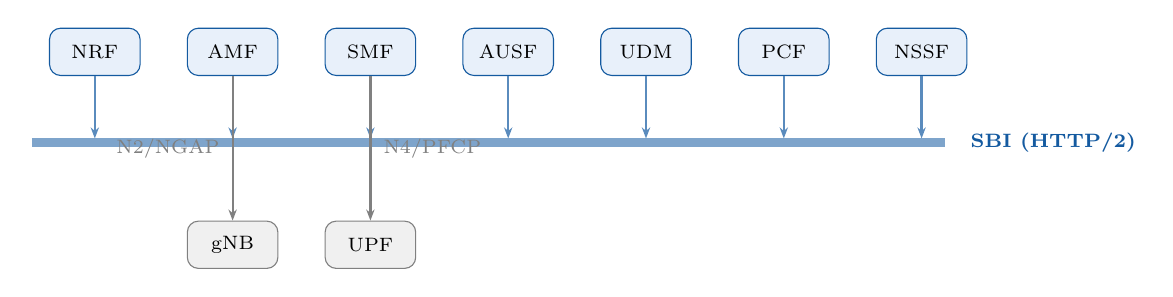
\begin{tikzpicture}[font=\scriptsize,
  nf/.style={rectangle, rounded corners, draw=accent, fill=light,
             minimum width=1.15cm, minimum height=0.6cm, align=center},
  ran/.style={rectangle, rounded corners, draw=gray, fill=gray!12,
              minimum width=1.15cm, minimum height=0.6cm, align=center},
  stub/.style={-{Stealth[length=1.4mm]}, thick, accent!70}]
  \draw[line width=3pt, accent!55] (0.2,0) -- (11.8,0);
  \node[accent, anchor=west] at (12.0,0) {\bfseries SBI (HTTP/2)};
  \foreach \x/\n in {1/NRF, 2.75/AMF, 4.5/SMF, 6.25/AUSF, 8/UDM, 9.75/PCF, 11.5/NSSF} {
    \node[nf] (\n) at (\x,1.15) {\n};
    \draw[stub] (\n) -- (\x,0.05);
  }
  \node[ran] (gnb) at (2.75,-1.3) {gNB};
  \node[ran] (upf) at (4.5,-1.3) {UPF};
  \draw[-{Stealth[length=1.4mm]}, thick, gray] (AMF) -- node[left=1pt]{N2/NGAP} (gnb);
  \draw[-{Stealth[length=1.4mm]}, thick, gray] (SMF) -- node[right=1pt]{N4/PFCP} (upf);
\end{tikzpicture}
\caption{5G Service-Based Architecture: every NF exposes and consumes services over the
common HTTP/2 SBI bus, while the RAN (N2/NGAP) and user plane (N4/PFCP) use point-to-point
interfaces.}
\label{fig:sba}
\end{figure}

\subsection{Why a From-Scratch Implementation Has Value}
Open-source 5G cores (open5GS, free5GC, OAI) already implement the basic 3GPP
procedures, so building yet another vanilla core has diminishing educational value.
This project is justified by \emph{what it adds}:

\begin{itemize}[leftmargin=1.4em]
  \item \textbf{Security posture:} none of the major OSS cores ship with mTLS between
        NFs, zero-trust network policies, or certificate lifecycle management --- a
        documented gap operators must patch themselves.
  \item \textbf{Roaming realism:} end-to-end SEPP/N32 roaming with topology hiding and
        message protection is largely missing from freely available cores, yet it is
        central to real operator deployments.
  \item \textbf{Testability:} the OSS ecosystem lacks a portable, scenario-driven
        conformance test framework; tests are run manually or with proprietary tooling.
  \item \textbf{Observability + security + BI fusion:} correlating Prometheus signalling
        metrics with anomaly detection and roaming business analytics is largely
        unexplored territory in the open-source 5G space.
\end{itemize}

\noindent\textbf{The prototype is the vehicle. The security architecture, roaming layer,
test framework, anomaly-detection engine, and BI reporting are the contributions.}

%==============================================================================
\section{Problem Statement}
The project addresses five engineering challenges, each with technical dimensions that
go beyond the baseline scope.

\begin{table}[h]
\centering
\footnotesize
\renewcommand{\arraystretch}{1.3}
\begin{tabularx}{\linewidth}{@{}c l X X@{}}
\toprule
\textbf{\#} & \textbf{Challenge} & \textbf{Baseline Scope} & \textbf{Extended Scope (This Project)}\\
\midrule
P1 & Protocol Complexity & Implement NGAP, NAS, HTTP/2 SBI correctly. &
  Add protocol-level security: SCTP over DTLS towards RAN, mTLS on all SBI calls.\\
P2 & Distributed Systems Design & NF registration, discovery, state coordination. &
  Add certificate-based NF identity via a lightweight PKI and token-based authorisation
  on SBI endpoints.\\
P3 & Roaming \& Interconnect & Single-PLMN core only. &
  Add SEPP + secured N32 interconnect, topology hiding, and home-routed / local-breakout
  roaming call flows across two PLMNs.\\
P4 & Deployment \& Observability & Docker Compose, Prometheus, Grafana. &
  Add network-policy enforcement (Cilium/eBPF), an anomaly-detection sidecar, a security
  event dashboard, and a BI reporting layer.\\
P5 & Standards Conformance & Interoperate with a RAN simulator. &
  Build a CI/CD-integrated conformance suite covering TS~23.502 registration, PDU session
  and roaming procedures.\\
\bottomrule
\end{tabularx}
\caption{Engineering challenges: baseline vs.\ extended scope.}
\label{tab:problems}
\end{table}

%==============================================================================
\section{Extended System Architecture}

\subsection{Minimal Viable Core (MVP)}
The MVP targets the minimum set of NFs required to demonstrate a complete 5G call flow.

\begin{table}[h]
\centering
\renewcommand{\arraystretch}{1.2}
\begin{tabularx}{\linewidth}{@{}l l X@{}}
\toprule
\textbf{NF} & \textbf{Scope} & \textbf{Role}\\
\midrule
\nf{NRF}  & Core    & Service registry \& discovery for all network functions.\\
\nf{AMF}  & Core    & Access \& Mobility Management --- SCTP/NGAP interface to the gNB.\\
\nf{SMF}  & Core    & Session Management --- PDU session lifecycle, user-plane control via PFCP.\\
\nf{UPF}  & Core    & User-Plane Forwarding --- GTP-U data path moving subscriber packets.\\
\nf{AUSF} & Core    & Authentication Server --- 5G-AKA and EAP-AKA$'$ procedures.\\
\nf{UDM}  & Core    & Unified Data Management --- subscriber profiles, authentication vectors.\\
\nf{PCF}  & Stretch & Policy control --- QoS rules, charging policies.\\
\nf{NSSF} & Stretch & Network slice selection.\\
\nf{SEPP} & Roaming & Security Edge Protection Proxy --- N32 interconnect to partner PLMNs.\\
\bottomrule
\end{tabularx}
\caption{Minimal Viable Core network functions (plus the SEPP for roaming).}
\label{tab:nfs}
\end{table}

\begin{figure}[h]
\centering
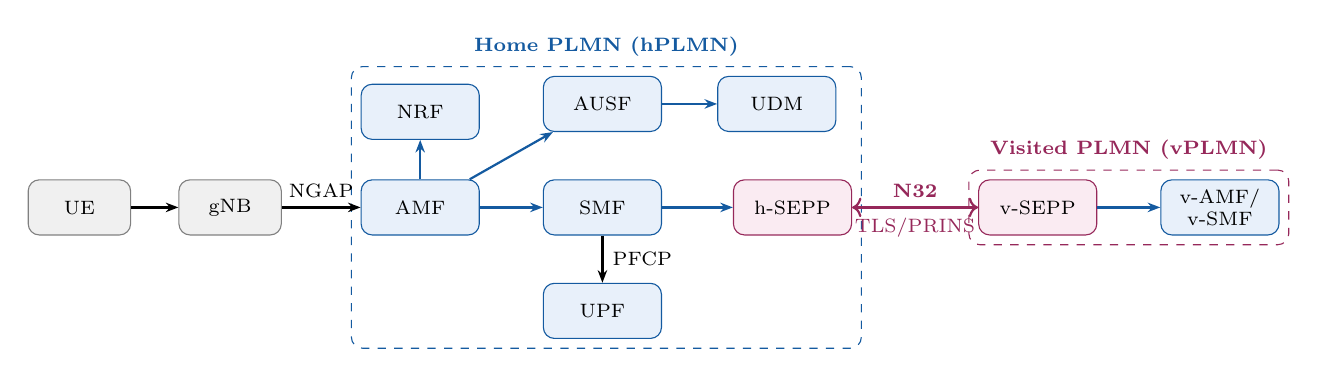
\begin{tikzpicture}[
  font=\scriptsize,
  nfbox/.style={rectangle, rounded corners, draw=accent, fill=light,
                minimum width=1.5cm, minimum height=0.7cm, align=center},
  sepp/.style={rectangle, rounded corners, draw=accent2, fill=light2,
               minimum width=1.5cm, minimum height=0.7cm, align=center},
  ran/.style={rectangle, rounded corners, draw=gray, fill=gray!12,
              minimum width=1.3cm, minimum height=0.7cm, align=center},
  arr/.style={-{Stealth[length=1.6mm]}, thick},
  sbi/.style={-{Stealth[length=1.6mm]}, thick, accent}]

  % home PLMN
  \node[ran]   (ue)  {UE};
  \node[ran, right=0.6cm of ue] (gnb) {gNB};
  \node[nfbox, right=1.0cm of gnb] (amf) {AMF};
  \node[nfbox, above=0.5cm of amf] (nrf) {NRF};
  \node[nfbox, right=0.8cm of amf] (smf) {SMF};
  \node[nfbox, below=0.6cm of smf] (upf) {UPF};
  \node[nfbox, above=0.6cm of smf] (ausf){AUSF};
  \node[nfbox, right=0.7cm of ausf](udm) {UDM};
  \node[sepp, right=0.9cm of smf]  (hsepp){h-SEPP};

  \draw[arr] (ue) -- (gnb);
  \draw[arr] (gnb) -- node[above]{NGAP} (amf);
  \draw[sbi] (amf) -- (smf);
  \draw[sbi] (amf) -- (nrf);
  \draw[sbi] (amf) -- (ausf);
  \draw[sbi] (ausf) -- (udm);
  \draw[arr] (smf) -- node[right]{PFCP} (upf);
  \draw[sbi] (smf) -- (hsepp);

  % visited PLMN
  \node[sepp, right=1.6cm of hsepp] (vsepp){v-SEPP};
  \node[nfbox, right=0.8cm of vsepp] (vamf){v-AMF/\\v-SMF};
  \draw[sbi, accent2, <->] (hsepp) -- node[above]{\bfseries N32}
        node[below]{TLS/PRINS} (vsepp);
  \draw[sbi] (vsepp) -- (vamf);

  \begin{scope}[on background layer]
    \node[draw=accent, dashed, rounded corners, fit=(nrf)(amf)(smf)(upf)(ausf)(udm)(hsepp),
          label=above:{\color{accent}\bfseries Home PLMN (hPLMN)}] {};
    \node[draw=accent2, dashed, rounded corners, fit=(vsepp)(vamf),
          label=above:{\color{accent2}\bfseries Visited PLMN (vPLMN)}] {};
  \end{scope}
\end{tikzpicture}
\caption{Extended architecture: single-PLMN SBA core plus SEPP/N32 roaming interconnect.
Blue links are mTLS-protected SBI; the magenta N32 link is secured between SEPPs.}
\label{fig:arch}
\end{figure}

\subsection{Security Layer --- Zero-Trust Architecture}
Zero-trust means no NF trusts another NF by default, regardless of network position.
Every inter-NF call must be authenticated and authorised.

\paragraph{Mutual TLS on the SBI.}
A lightweight internal PKI (Vault or a self-hosted CA) issues X.509 certificates per NF
instance. All HTTP/2 SBI calls require client-certificate presentation; a server rejects
any call from an uncertified peer. Certificate rotation is automated and tested in the
deployment pipeline.

\paragraph{OAuth2 / JWT Token Authorisation (TS 33.501 §13).}
The NRF acts as an OAuth2 authorisation server, issuing access tokens scoped to specific
NF service operations. The AMF, SMF, and UDM validate tokens on every inbound SBI
request; a missing or expired token yields HTTP~401. Token scopes map directly to 3GPP
NF service names (e.g.\ \code{namf-comm}, \code{nsmf-pdusession}).

\paragraph{Network Policy Enforcement.}
Kubernetes Network Policies (or Cilium L7 policies) enforce that only permitted NF pairs
communicate. The AMF cannot reach the UPF directly; all data-plane control goes through
the SMF via PFCP --- enforced at the network layer, not by convention. eBPF-based
inspection provides per-flow visibility without kernel-module overhead.

\paragraph{Secrets Management.}
Database credentials, certificate private keys, and IMSI encryption keys are never stored
in environment variables or Compose files. HashiCorp Vault provides dynamic secret
injection at container startup, and all secret access is logged and audited.

\begin{quote}\itshape
Security anti-pattern to explicitly avoid: storing subscriber IMSI or authentication
vectors in plaintext in MongoDB. UDM data at rest is encrypted using MongoDB Client-Side
Field Level Encryption (CSFLE).
\end{quote}

\begin{figure}[h]
\centering
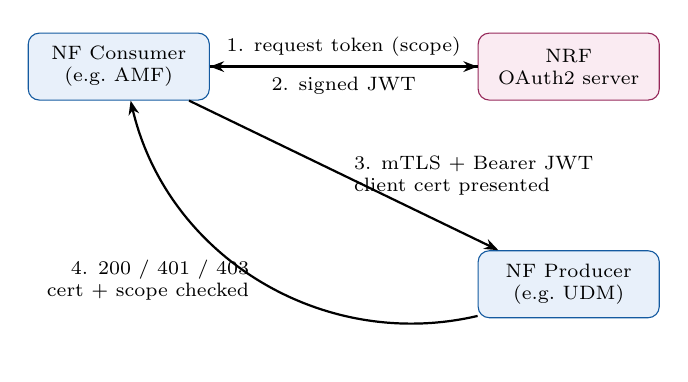
\begin{tikzpicture}[font=\scriptsize,
  box/.style={rectangle, rounded corners, draw=accent, fill=light,
              minimum width=2.3cm, minimum height=0.85cm, align=center},
  nrf/.style={rectangle, rounded corners, draw=accent2, fill=light2,
              minimum width=2.3cm, minimum height=0.85cm, align=center},
  a/.style={-{Stealth[length=1.8mm]}, thick}]
  \node[box] (cons) {NF Consumer\\{\scriptsize (e.g.\ AMF)}};
  \node[nrf, right=3.4cm of cons] (nrf) {NRF\\{\scriptsize OAuth2 server}};
  \node[box, below=1.9cm of nrf] (prod) {NF Producer\\{\scriptsize (e.g.\ UDM)}};
  \draw[a] (cons) -- node[above]{1. request token (scope)} (nrf);
  \draw[a] (nrf) -- node[below]{2. signed JWT} (cons);
  \draw[a] (cons) -- node[right, align=left]
        {3. mTLS + Bearer JWT\\{\scriptsize client cert presented}} (prod);
  \draw[a] (prod) to[bend left=45] node[left, align=right]
        {4. 200 / 401 / 403\\{\scriptsize cert + scope checked}} (cons);
\end{tikzpicture}
\caption{Zero-trust SBI call: the consumer obtains a scoped OAuth2 token from the NRF, then
calls the producer over mutual TLS; the producer verifies both the client certificate and
the token scope before responding.}
\label{fig:zerotrust}
\end{figure}

\subsection{Roaming and Interconnect Layer}
\label{sec:roaming}
Roaming lets a subscriber of the \textbf{home PLMN (hPLMN)} obtain service while attached
to a \textbf{visited PLMN (vPLMN)}. In the SBA, the two networks never expose their
internal NFs directly to each other; instead, each operator places a \textbf{Security
Edge Protection Proxy (SEPP)} at its boundary, and the SEPPs interconnect over the
\textbf{N32} reference point.

\paragraph{SEPP and the N32 interface.}
\begin{itemize}[leftmargin=1.4em]
  \item \textbf{N32-c (control):} a TLS-protected control channel where the two SEPPs
        perform capability negotiation and agree on the security mechanism.
  \item \textbf{N32-f (forwarding):} the channel that carries the actual inter-PLMN SBI
        messages, protected either by TLS or by \textbf{PRINS} (PRotocol for N32
        INterconnect Security), which allows authorised IPX intermediaries to modify only
        permitted fields while integrity/confidentiality of the rest is preserved via
        JWS/JWE.
  \item \textbf{Topology hiding:} the SEPP rewrites internal NF identifiers so the partner
        network never learns the home operator's internal topology.
\end{itemize}

\paragraph{Roaming models supported.}
\begin{itemize}[leftmargin=1.4em]
  \item \textbf{Home-Routed (HR):} the user plane is anchored in the hPLMN. The vSMF in the
        visited network coordinates with the hSMF/hUPF via N16/SBI over N32. Used when the
        home operator must retain control of the data path (lawful intercept, policy,
        charging).
  \item \textbf{Local Breakout (LBO):} the user plane is anchored in the vPLMN (vUPF), with
        policy/charging still governed by the hPLMN's PCF. Lower latency, closer to the
        user.
\end{itemize}

\paragraph{Roaming procedures (TS 23.502).} The layer implements roaming registration
(authentication vectors fetched from the home UDM/AUSF via the SEPP) and a roaming PDU
session establishment for at least one of the two models, validated by the conformance
suite (see \code{ROAM-01/02} in Section~\ref{sec:tests}).

\begin{figure}[h]
\centering
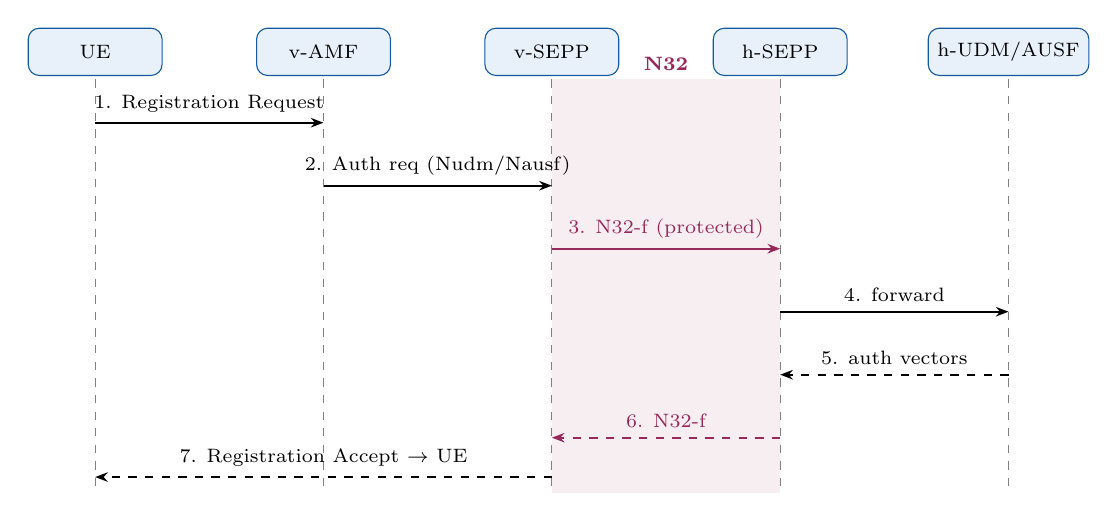
\begin{tikzpicture}[font=\scriptsize,
  part/.style={rectangle, rounded corners, draw=accent, fill=light,
               minimum width=1.7cm, minimum height=0.6cm, align=center},
  msg/.style={-{Stealth[length=1.6mm]}, thick},
  ret/.style={-{Stealth[length=1.6mm]}, thick, dashed}]
  \def\yb{-5.6}
  \foreach \x/\name/\id in {0/UE/ue, 2.9/{v-AMF}/vamf, 5.8/{v-SEPP}/vsepp,
                            8.7/{h-SEPP}/hsepp, 11.6/{h-UDM/AUSF}/hudm} {
    \node[part] (\id) at (\x,0) {\name};
    \draw[gray, dashed] (\x,-0.35) -- (\x,\yb);
  }
  \begin{scope}[on background layer]
    \fill[accent2!8] (5.8,-0.35) rectangle (8.7,\yb);
    \node[accent2, font=\scriptsize] at (7.25,-0.15) {\bfseries N32};
  \end{scope}
  \draw[msg] (0,-0.9)   -- node[above]{1. Registration Request} (2.9,-0.9);
  \draw[msg] (2.9,-1.7) -- node[above]{2. Auth req (Nudm/Nausf)} (5.8,-1.7);
  \draw[msg, accent2] (5.8,-2.5) -- node[above]{3. N32-f (protected)} (8.7,-2.5);
  \draw[msg] (8.7,-3.3) -- node[above]{4. forward} (11.6,-3.3);
  \draw[ret] (11.6,-4.1)-- node[above]{5. auth vectors} (8.7,-4.1);
  \draw[ret, accent2] (8.7,-4.9)-- node[above]{6. N32-f} (5.8,-4.9);
  \draw[ret] (5.8,-5.4) -- node[above]{7. Registration Accept $\rightarrow$ UE} (0,-5.4);
\end{tikzpicture}
\caption{Home-routed roaming registration: the visited network reaches the home UDM/AUSF
only through the SEPP pair over the secured N32 interface (topology hiding, message
protection).}
\label{fig:roaming-seq}
\end{figure}

\paragraph{Why roaming matters for security and BI.} Roaming is both a
\emph{security surface} (fake partner networks, N32 message tampering, IPX abuse) and a
\emph{business dimension} (which visited networks carry the operator's subscribers, at
what volume and success rate). It therefore feeds directly into the anomaly-detection
engine (Section~\ref{sec:anomaly}) and the observability/BI layer
(Section~\ref{sec:observability}).

\subsection{Anomaly Detection Engine}
\label{sec:anomaly}
A lightweight anomaly-detection sidecar runs alongside the core, consuming the Prometheus
metrics stream and applying statistical and ML-based detection to identify abnormal
signalling patterns.

\begin{table}[h]
\centering
\footnotesize
\renewcommand{\arraystretch}{1.3}
\begin{tabularx}{\linewidth}{@{}l X X@{}}
\toprule
\textbf{Threat} & \textbf{Observable Signal} & \textbf{Detection Method}\\
\midrule
Rogue UE / IMSI enumeration & Abnormal registration burst from a single location &
  Rate-based threshold + z-score on registration-count time series.\\
IMSI Catcher (fake gNB) & gNB authenticates, then requests identity without AKA &
  NAS message-sequence anomaly detection (HMM or rule-based FSM).\\
Session Hijacking & SMF receives \emph{modify session} for a session not in its state &
  State correlation across SMF and UDM logs.\\
DoS on AMF & Registration-request flood from a single PLMN or TA &
  Sliding-window rate limiter with AMF-level circuit breaker.\\
\textbf{Roaming abuse / fraud} & Sudden spike of registrations from an unusual visited PLMN,
  or N32 messages failing integrity checks &
  Per-PLMN baseline + z-score; N32 JWS/JWE verification-failure counter.\\
\bottomrule
\end{tabularx}
\caption{Threat models addressed by the anomaly-detection engine (including roaming).}
\label{tab:threats}
\end{table}

\paragraph{Implementation approach.}
\begin{itemize}[leftmargin=1.4em]
  \item \textbf{Phase 1 (Wks 9--10):} rule-based detection using Prometheus alerting rules
        --- fast to implement, covers the most common threats.
  \item \textbf{Phase 2 (Wks 11--12):} statistical anomaly detection using z-score and IQR
        on registration and session-count (and per-PLMN roaming) time series.
  \item \textbf{Phase 3 (stretch):} train a lightweight isolation forest or LSTM on captured
        signalling traces to detect subtle sequence anomalies.
\end{itemize}
\emph{Practical scope check:} Phases 1--2 are achievable within the internship timeline;
Phase 3 is a stretch goal that adds research value without blocking delivery.

\begin{figure}[h]
\centering
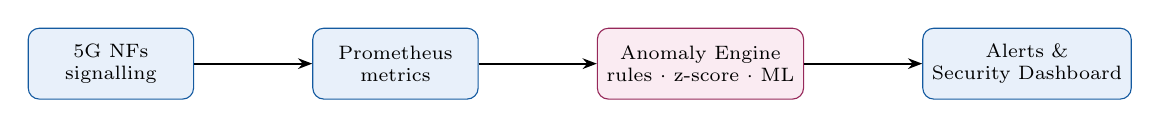
\begin{tikzpicture}[font=\scriptsize, node distance=1.5cm,
  b/.style={rectangle, rounded corners, draw=accent, fill=light,
            minimum width=2.1cm, minimum height=0.9cm, align=center},
  d/.style={rectangle, rounded corners, draw=accent2, fill=light2,
            minimum width=2.5cm, minimum height=0.9cm, align=center},
  a/.style={-{Stealth[length=1.8mm]}, thick}]
  \node[b] (nf) {5G NFs\\{\scriptsize signalling}};
  \node[b, right=of nf] (prom) {Prometheus\\{\scriptsize metrics}};
  \node[d, right=of prom] (eng) {Anomaly Engine\\{\scriptsize rules $\cdot$ z-score $\cdot$ ML}};
  \node[b, right=of eng] (out) {Alerts \&\\Security Dashboard};
  \draw[a] (nf) -- (prom);
  \draw[a] (prom) -- (eng);
  \draw[a] (eng) -- (out);
\end{tikzpicture}
\caption{Anomaly-detection pipeline: signalling metrics flow from the NFs through Prometheus
to the detection sidecar, which raises alerts on the security dashboard.}
\label{fig:anomaly-pipe}
\end{figure}

%==============================================================================
\section{Observability and Business Intelligence}
\label{sec:observability}
Observability and BI are treated as one continuous pipeline: low-level signals are
collected, correlated for \emph{operational} insight, then aggregated for \emph{business}
insight.

\subsection{Observability pipeline}
\begin{table}[h]
\centering
\renewcommand{\arraystretch}{1.2}
\begin{tabularx}{\linewidth}{@{}l l X@{}}
\toprule
\textbf{Concern} & \textbf{Tooling} & \textbf{Flow}\\
\midrule
Metrics & Prometheus + Grafana & Scrape each NF's \code{/metrics}; NF KPI + security dashboards.\\
Logs    & Fluent Bit + Loki    & Structured NF logs shipped to Loki, correlated by trace id.\\
Traces  & OpenTelemetry + Tempo/Jaeger & End-to-end SBI call traces across NFs (stretch).\\
Packets & Wireshark / tcpdump  & pcap evidence for conformance tests and fault analysis.\\
\bottomrule
\end{tabularx}
\caption{Observability pipelines.}
\label{tab:obs}
\end{table}

\begin{figure}[h]
\centering
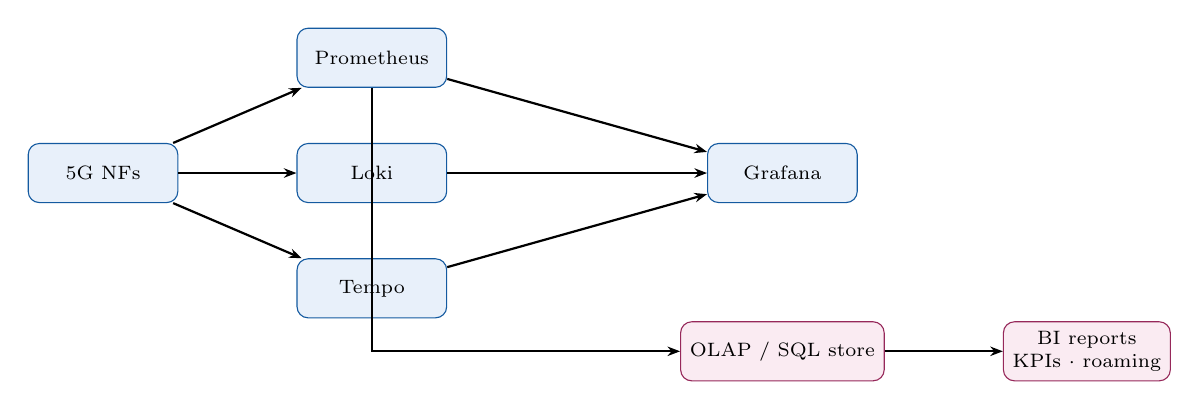
\begin{tikzpicture}[font=\scriptsize, node distance=0.7cm and 1.5cm,
  b/.style={rectangle, rounded corners, draw=accent, fill=light,
            minimum width=1.9cm, minimum height=0.75cm, align=center},
  bi/.style={rectangle, rounded corners, draw=accent2, fill=light2,
             minimum width=1.9cm, minimum height=0.75cm, align=center},
  a/.style={-{Stealth[length=1.6mm]}, thick}]
  \node[b] (nf) {5G NFs};
  \node[b, above right=of nf] (prom) {Prometheus};
  \node[b, right=of nf] (loki) {Loki};
  \node[b, below right=of nf] (tempo) {Tempo};
  \node[b, right=3.3cm of loki] (graf) {Grafana};
  \node[bi, below=1.5cm of graf] (olap) {OLAP / SQL store};
  \node[bi, right=of olap] (report) {BI reports\\{\scriptsize KPIs $\cdot$ roaming}};
  \draw[a] (nf) -- (prom);  \draw[a] (nf) -- (loki);  \draw[a] (nf) -- (tempo);
  \draw[a] (prom) -- (graf); \draw[a] (loki) -- (graf); \draw[a] (tempo) -- (graf);
  \draw[a] (prom) |- (olap); \draw[a] (olap) -- (report);
\end{tikzpicture}
\caption{Observability-to-BI pipeline: metrics, logs and traces feed operational dashboards
in Grafana, while aggregated metrics are materialised into an OLAP/SQL store that drives the
business-intelligence reports (including roaming analytics).}
\label{fig:obs-bi}
\end{figure}

\subsection{Business-Intelligence (BI) reporting layer}
On top of raw observability, a BI layer periodically aggregates signalling metrics into a
reporting store (e.g.\ Prometheus recording rules $\rightarrow$ a relational/OLAP store)
and produces operator-oriented dashboards and scheduled reports. Representative KPIs:

\begin{table}[h]
\centering
\footnotesize
\renewcommand{\arraystretch}{1.25}
\begin{tabularx}{\linewidth}{@{}l l X@{}}
\toprule
\textbf{KPI domain} & \textbf{Example metric} & \textbf{Business question answered}\\
\midrule
Registration & Registration success ratio, attach latency p95 & Is onboarding healthy?\\
Sessions     & PDU session setup success, active sessions & Is the data service usable?\\
Security     & Anomaly alerts/day, cert-expiry countdown & Is the core under attack / compliant?\\
\textbf{Roaming (in)}  & Inbound roamers by visited PLMN, HR vs LBO split &
  Which partners bring subscribers, and how?\\
\textbf{Roaming (out)} & Outbound roaming success ratio, N32 handshake success &
  Are our subscribers served abroad reliably?\\
\textbf{Roaming quality} & Inter-PLMN signalling latency, N32 failure rate &
  Which roaming partners degrade experience?\\
\bottomrule
\end{tabularx}
\caption{Business-intelligence KPIs, with dedicated roaming analytics.}
\label{tab:bi}
\end{table}

The BI layer materialises three deliverable artefacts: (i)~a \textbf{NF KPI dashboard},
(ii)~a \textbf{security event dashboard} (alert timeline, anomaly counts, certificate
expiry), and (iii)~a \textbf{roaming analytics dashboard \& periodic report} (top visited
PLMNs, roaming success ratios, N32 health, home-routed vs local-breakout distribution).

%==============================================================================
\section{Automated Conformance Test Framework}
\label{sec:tests}
The test framework is a first-class deliverable. It validates the implementation against
3GPP procedures, enables CI/CD regression testing, and demonstrates the core's security
and roaming posture under adversarial scenarios.

\subsection{Test architecture}
\begin{itemize}[leftmargin=1.4em]
  \item \textbf{Test runner:} Go-based, reusing the core's codebase for protocol familiarity.
  \item \textbf{Scenario format:} YAML test cases specifying message sequences, expected
        responses, and timing constraints.
  \item \textbf{Execution:} Docker Compose brings up the full core + RAN simulator; the
        runner executes scenarios and reports pass/fail with pcap evidence.
  \item \textbf{CI/CD:} GitHub Actions runs the suite on every commit; a failing conformance
        test blocks merge.
\end{itemize}

\begin{figure}[h]
\centering
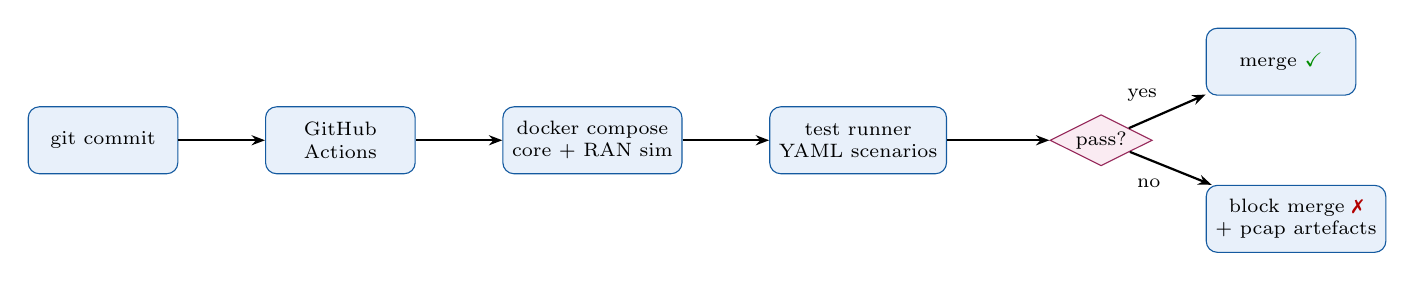
\begin{tikzpicture}[font=\scriptsize, node distance=1.1cm,
  s/.style={rectangle, rounded corners, draw=accent, fill=light,
            minimum width=1.9cm, minimum height=0.85cm, align=center},
  dec/.style={diamond, aspect=2, draw=accent2, fill=light2, align=center, inner sep=1pt},
  a/.style={-{Stealth[length=1.7mm]}, thick}]
  \node[s] (commit) {git commit};
  \node[s, right=of commit] (ci) {GitHub\\Actions};
  \node[s, right=of ci] (up) {docker compose\\core + RAN sim};
  \node[s, right=of up] (run) {test runner\\{\scriptsize YAML scenarios}};
  \node[dec, right=1.3cm of run] (pass) {pass?};
  \node[s, above right=0.4cm and 1cm of pass] (merge) {merge \yes};
  \node[s, below right=0.4cm and 1cm of pass] (block) {block merge \no\\{\scriptsize + pcap artefacts}};
  \draw[a] (commit) -- (ci); \draw[a] (ci) -- (up);
  \draw[a] (up) -- (run);    \draw[a] (run) -- (pass);
  \draw[a] (pass) -- node[above left]{yes} (merge);
  \draw[a] (pass) -- node[below left]{no} (block);
\end{tikzpicture}
\caption{CI/CD conformance flow: every commit spins up the full core plus RAN simulator, runs
the YAML scenarios, and gates the merge on the result --- with pcap evidence on failure.}
\label{fig:cicd}
\end{figure}

\begin{table}[h]
\centering
\footnotesize
\renewcommand{\arraystretch}{1.25}
\begin{tabularx}{\linewidth}{@{}l l l X@{}}
\toprule
\textbf{TC-ID} & \textbf{Test Case} & \textbf{Procedure} & \textbf{Pass Criterion}\\
\midrule
TC-01   & Initial UE Registration       & TS 23.502 §4.2.2.2 & Registration Accept within 2s.\\
TC-02   & 5G-AKA Authentication         & §4.6.2             & RAND/AUTN sent, RES* verified, SEAF key derived.\\
TC-03   & PDU Session Establishment     & §4.3.2             & N1 PDU Session Accept, GTP-U tunnel active.\\
TC-04   & UE Deregistration             & §4.2.2.3           & All sessions released, AMF state cleared.\\
TC-05   & Handover (Xn) \emph{(stretch)}& §4.9.1.2           & UE context transferred, GTP-U path switched.\\
\textbf{ROAM-01} & Roaming Registration (HR) & §4.2.2.2 (roaming) &
  Home-routed registration via SEPP/N32; auth vectors fetched from home UDM.\\
\textbf{ROAM-02} & Roaming PDU Session (LBO) & §4.3.2 (roaming) &
  Local-breakout session with vUPF anchor; home PCF policy applied.\\
SEC-01  & mTLS enforcement (no cert)    & TS 33.501 §13      & SBI call rejected with TLS handshake failure.\\
SEC-02  & Token scope violation         & §13.3              & AMF$\rightarrow$UDM with wrong scope returns HTTP 403.\\
SEC-03  & IMSI enumeration attempt      & Threat model       & Anomaly engine alerts within 10 registration probes.\\
\textbf{SEC-04} & N32 message tampering  & TS 33.501 (SEPP)  & Modified N32-f payload fails JWS/JWE verification.\\
PERF-01 & Registration throughput       & KPI baseline       & $\geq$50 concurrent registrations without error.\\
PERF-02 & PDU session latency           & KPI baseline       & p95 session-establishment latency $\leq$500\,ms under load.\\
\bottomrule
\end{tabularx}
\caption{Conformance, roaming, security and performance test cases.}
\label{tab:testcases}
\end{table}

\subsection{Fault-injection scenarios}
\begin{itemize}[leftmargin=1.4em]
  \item \textbf{NF crash recovery:} kill the SMF mid-session; verify the AMF detects NF
        deregistration via NRF heartbeat timeout and that session cleanup occurs.
  \item \textbf{Database unavailability:} disconnect MongoDB; verify UDM returns 503 rather
        than hanging.
  \item \textbf{Certificate expiry:} expire the AMF certificate; verify its SBI calls are
        rejected until the certificate is rotated.
  \item \textbf{Network partition:} isolate the UPF from the SMF via network policy; verify
        PFCP keepalive triggers session teardown within the timeout.
  \item \textbf{Roaming partner outage:} drop the N32 link to the vPLMN; verify roaming
        registrations fail gracefully and the roaming dashboard flags the partner down.
\end{itemize}

%==============================================================================
\section{Methodology and Work Plan}
The work follows an incremental, milestone-driven approach across six phases over a
4--6 month internship. Security, roaming and testing are built in from Phase~2 onwards ---
not bolted on at the end.

\begin{table}[h]
\centering
\footnotesize
\renewcommand{\arraystretch}{1.3}
\begin{tabularx}{\linewidth}{@{}c l l X@{}}
\toprule
\textbf{Phase} & \textbf{Weeks} & \textbf{Title} & \textbf{Activities}\\
\midrule
P1 & 1--2   & State of the Art &
  5G SBA study (R15/R16); survey open5GS, free5GC, OAI; identify security \& roaming gaps;
  define PKI, roaming model and threat model.\\
P2 & 3--4   & Architecture \& Security Design &
  System architecture; SBI API contracts; data models; PKI design; NF identity; SEPP/N32
  design; MongoDB CSFLE; Vault integration plan.\\
P3 & 5--10  & Core Implementation &
  Implement NRF, AMF, SMF, UPF, AUSF, UDM in Go; deploy internal PKI; add mTLS + OAuth2 on
  all SBI endpoints; subscriber DB with CSFLE.\\
P4 & 11--14 & Integration, Roaming \& Test Framework &
  Integrate RAN/UE simulator; implement SEPP/N32 roaming (ROAM-01/02); build the
  conformance framework (TC-01--PERF-02); rule-based + statistical anomaly detection;
  CI/CD pipeline.\\
P5 & 15--18 & Deployment, Observability \& BI &
  Docker Compose orchestration; optional Kubernetes + Helm; Cilium network policies;
  Prometheus + Grafana; security event + roaming analytics dashboards; BI reporting.\\
P6 & 19--24 & Validation \& Documentation &
  Full conformance run; load testing (PERF-01/02); fault injection; anomaly \& roaming
  validation; final report and live demonstration.\\
\bottomrule
\end{tabularx}
\caption{Six-phase, milestone-driven work plan.}
\label{tab:plan}
\end{table}

\begin{figure}[h]
\centering
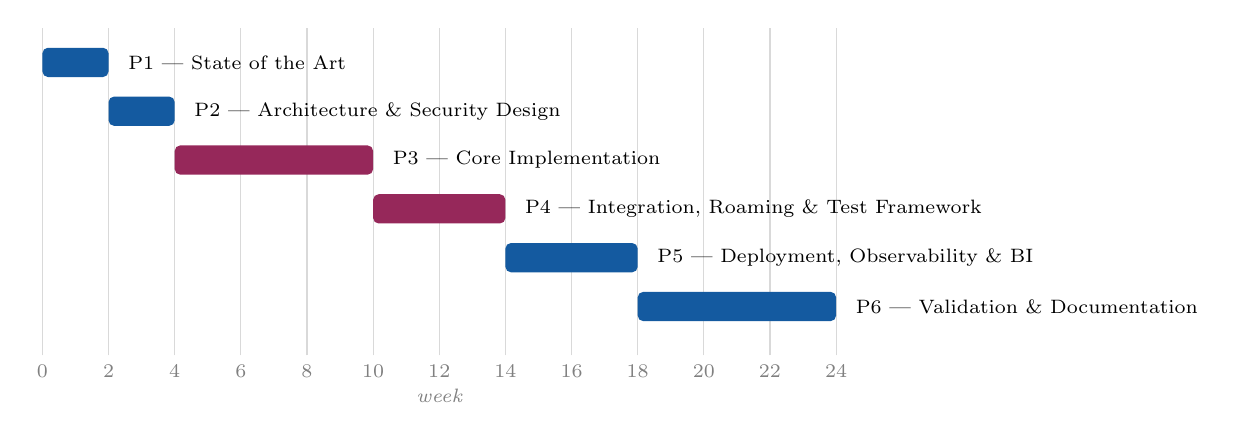
\begin{tikzpicture}[font=\scriptsize, x=0.42cm, y=0.62cm]
  \foreach \w in {0,2,...,24} {
    \draw[gray!30] (\w,0) -- (\w,6.7);
    \node[gray, below] at (\w,0) {\w};
  }
  \node[gray, below=3mm] at (12,0) {\itshape week};
  \newcommand{\gbar}[5]{%
    \fill[#4, rounded corners=2pt] (#1,#3-0.3) rectangle (#2,#3+0.3);
    \node[anchor=west, black] at (#2+0.3,#3) {#5};}
  \gbar{0}{2}{6}{accent}{P1 — State of the Art}
  \gbar{2}{4}{5}{accent}{P2 — Architecture \& Security Design}
  \gbar{4}{10}{4}{accent2}{P3 — Core Implementation}
  \gbar{10}{14}{3}{accent2}{P4 — Integration, Roaming \& Test Framework}
  \gbar{14}{18}{2}{accent}{P5 — Deployment, Observability \& BI}
  \gbar{18}{24}{1}{accent}{P6 — Validation \& Documentation}
\end{tikzpicture}
\caption{Indicative 24-week Gantt chart of the six-phase work plan.}
\label{fig:gantt}
\end{figure}

%==============================================================================
\section{Technical Environment}
\begin{table}[h]
\centering
\footnotesize
\renewcommand{\arraystretch}{1.25}
\begin{tabularx}{\linewidth}{@{}l X@{}}
\toprule
\textbf{Category} & \textbf{Tools \& Technologies}\\
\midrule
Languages     & Go (primary --- NFs, test runner), C (UPF data path / eBPF), Shell, optional TypeScript (security/roaming dashboard UI).\\
Protocols     & NGAP, NAS-5GS, PFCP, GTP-U, HTTP/2 (SBI), \textbf{N32}, SCTP (over DTLS), OAuth2/JWT, TLS 1.3.\\
Security      & HashiCorp Vault (secrets), cert-manager / CFSSL (PKI), Cilium (network policy + eBPF), MongoDB CSFLE (data at rest), SEPP (N32 protection).\\
Data          & MongoDB 7.x with CSFLE; Redis (session-state cache); relational/OLAP store for BI reporting.\\
Containers    & Docker, Docker Compose (primary), Kubernetes + Helm (stretch).\\
Observability \& BI & Prometheus, Grafana, Loki, Tempo/Jaeger (stretch), Wireshark/tcpdump; BI dashboards \& scheduled reports.\\
Testing       & Custom Go test runner, YAML scenarios, GitHub Actions CI/CD, k6 (load testing).\\
RAN Simulation& UERANSIM (primary) or OAI gNB/UE; software gNB + multiple virtual UEs.\\
Platform      & Linux (Ubuntu 22.04 LTS, VM or WSL2); kernel GTP module for UPF; min.\ 16\,GB RAM, 8 CPU cores.\\
Tooling       & Git/GitHub, Make, VS Code + Go, Protobuf (optional NF-internal messaging).\\
\bottomrule
\end{tabularx}
\caption{Technical environment.}
\label{tab:env}
\end{table}

%==============================================================================
\section{Expected Deliverables}
\begin{table}[h]
\centering
\footnotesize
\renewcommand{\arraystretch}{1.3}
\begin{tabularx}{\linewidth}{@{}c l X@{}}
\toprule
\textbf{\#} & \textbf{Deliverable} & \textbf{Description}\\
\midrule
D1 & Architecture \& API Specification & Architecture diagrams, SBI API contracts (OpenAPI 3.0), PKI design, SEPP/N32 roaming design, threat-model document.\\
D2 & Working 5G Core MVP & NRF, AMF, SMF, UPF, AUSF, UDM in Go with full mTLS + OAuth2 and MongoDB CSFLE.\\
D3 & Roaming Interconnect & SEPP + secured N32; home-routed and/or local-breakout roaming validated by ROAM-01/02.\\
D4 & Conformance Test Suite & Go runner + YAML scenarios covering TC-01--PERF-02 (incl.\ roaming \& security); CI/CD integrated.\\
D5 & Anomaly Detection Engine & Rule-based + statistical sidecar; validated against $\geq$3 threat scenarios (SEC-01--SEC-04).\\
D6 & Containerised Deployment & Docker Compose with Vault, PKI, all NFs, SEPP, RAN simulator; optional Kubernetes + Helm.\\
D7 & Observability \& BI Stack & Prometheus + Grafana with NF KPI, security event and \textbf{roaming analytics} dashboards; scheduled BI reports.\\
D8 & Technical Documentation \& Final Report & Architecture guide, deployment guide, test results, security analysis, roaming report, lessons learned, live demo.\\
\bottomrule
\end{tabularx}
\caption{Expected deliverables.}
\label{tab:deliverables}
\end{table}

%==============================================================================
\section{Skills to Be Developed}
\begin{table}[h]
\centering
\footnotesize
\renewcommand{\arraystretch}{1.25}
\begin{tabularx}{\linewidth}{@{}l X@{}}
\toprule
\textbf{Skill Area} & \textbf{Specific Competencies}\\
\midrule
5G Standards        & 3GPP R15+ SBA; NF roles; NGAP/NAS/PFCP/GTP-U/SBI/\textbf{N32} stack; TS 23.502 call flows (incl.\ roaming); TS 33.501 security.\\
Distributed Systems & Micro-services in Go; service discovery; state coordination; fault tolerance; circuit breakers; distributed tracing.\\
Telecom Security    & PKI, mTLS, OAuth2/JWT, zero-trust networking, 5G-AKA, IMSI protection, \textbf{SEPP/N32 interconnect security}, threat modelling.\\
Cloud-Native Ops    & Docker, Kubernetes, Helm, Cilium/eBPF, Vault secrets management, CI/CD pipelines.\\
Observability \& BI & Prometheus metric design, Grafana dashboards, anomaly-detection algorithms, time-series analysis, \textbf{roaming KPI \& BI reporting}.\\
Test Engineering    & Protocol conformance testing, scenario-based frameworks, fault injection, load testing, pcap evidence capture.\\
\bottomrule
\end{tabularx}
\caption{Targeted competencies.}
\label{tab:skills}
\end{table}

%==============================================================================
\section{Feasibility and Scope Justification}

\subsection{Why this scope is achievable}
The project is structured around a strict MVP core (P3) that must be complete before any
extended feature is added. The security layer is incremental: mTLS and OAuth2 are standard
Go library features, not novel research. Roaming reuses the same SBI stack across a SEPP
proxy rather than a new protocol implementation. The test framework is Go code calling the
same NF HTTP endpoints already built --- there is no second protocol stack to implement.

\subsection{Risk register}
\begin{table}[h]
\centering
\footnotesize
\renewcommand{\arraystretch}{1.3}
\begin{tabularx}{\linewidth}{@{}X c X@{}}
\toprule
\textbf{Risk} & \textbf{Likelihood} & \textbf{Mitigation}\\
\midrule
NGAP/NAS complexity blocks AMF delivery & Medium &
  Use UERANSIM's NGAP library as reference; allocate 2 extra days per NF in P3.\\
PKI integration delays core development & Low &
  Use CFSSL or cert-manager with pre-built image; PKI is a one-day task with tooling.\\
Roaming (SEPP/N32) adds too much scope & Medium &
  Implement one roaming model end-to-end (home-routed \emph{or} local-breakout); the second
  is a stretch. N32 can start with TLS before PRINS.\\
Anomaly detection Phase 3 (ML) out of reach & High &
  Phase 3 is explicitly a stretch; Phases 1--2 suffice for the deliverable.\\
RAN simulator compatibility issues & Low &
  UERANSIM is the most widely tested OSS RAN simulator; fallback to OAI gNB.\\
Kubernetes track adds too much scope & Medium &
  Kubernetes is optional; Docker Compose is the primary target and covers all deliverables.\\
\bottomrule
\end{tabularx}
\caption{Risk register.}
\label{tab:risks}
\end{table}

\subsection{Commercial potential (long-term)}
While this is an internship project, the architecture points toward commercially relevant
directions: a security-hardened, roaming-capable 5G-core \emph{testbed-as-a-service} would
address a real gap (vendors and MVNOs pay for on-demand isolated test environments); the
conformance suite could become a standalone product for NF vendors; and the anomaly-detection
engine addresses the 5G network-security-monitoring market (projected at \$4.5B by 2028).

\begin{quote}\itshape
Important caveat: the internship scope must remain an internship scope. These directions
frame the project's relevance, not to expand the deliverables. Scope discipline is what
makes the project succeed.
\end{quote}

%==============================================================================
\section{Chapter Conclusion}
This chapter established the ambition, context, and boundaries of the project: a
cloud-native 5G Core built \emph{from scratch}, but differentiated by five engineering
contributions --- zero-trust security, SEPP/N32 roaming, anomaly detection, a fused
observability/BI layer, and an automated conformance test framework. It fixed a strict MVP,
a phased and risk-managed work plan, a concrete technical environment, and a clear set of
deliverables. The following chapters (Part Two onward) will document, in development order,
the detailed design, the implementation of each network function and the roaming
interconnect, the security hardening, the test and BI results, and the final validation.

\end{document}
